\documentclass[12pt]{article}                         
\pagestyle{plain}

\usepackage{amsmath}     % Enhanced math environments (e.g., align).
\usepackage{amsfonts}    % Math fonts (e.g., \mathfrak{}).
\usepackage{amstext}     % Text inside math mode (e.g., \text{where}).
\usepackage{amssymb}     % Extra math symbols (e.g., \mathbb{R}).
\usepackage{array}       % Advanced table/array column definitions.
\usepackage{circledtext} % Puts text inside a circle (e.g., \circledtext{A}).
\usepackage{comment}     % Include/exclude blocks of text.
\usepackage{enumerate}   % Customize itemized/numbered lists.
\usepackage{graphicx}    % Include images/graphics (\includegraphics).
\usepackage{latexsym}    % Access to basic LaTeX symbols.
\usepackage{multicol}    % Allows text columns on a page.
\usepackage{pgfplots}    % Create scientific plots from data (based on TikZ).
\usepackage{tabularx}    % Tables that stretch to page width.
\usepackage{tasks}       % Create multi-column lists.
\usepackage{textcomp}    % Provides many text symbols (e.g., \textcelsius).
\usepackage{tikz}        % Create vector graphics and diagrams.
\usepackage{xcolor}      % Define and use colors.
\usepackage{fancyhdr}
\usepackage{tcolorbox}
\usepackage{enumitem}

\usepackage[
  letterpaper,
  left=0.8in,
  right=0.8in,
  textheight=9.5in,
  bmargin=0.5in  % Adjust this value to push the footer down
]{geometry}
\pagestyle{fancy}
\fancyhf{} % Clear all header and footer fields
\fancyhead[L]{Your Name:} % Left header with name
\fancyhead[R]{Novemeber 18th 2025} % Right header with date
\renewcommand{\headrulewidth}{0.4pt} % Horizontal line below the header

\begin{document}

% Main title
\begin{center}
    \Large \textbf{Math 115E Activity XX} \\
    \vspace{0.2cm}
    \normalsize Old Activity 11-5 and 11-7
\end{center}
\vspace{-0.5cm}
\subsection*{Graphing Quadratic Functions}
\begin{tcolorbox}[
    width=\linewidth,
    colframe=black,         % Border color
    colback=white,          % Background color
    boxrule=0.5pt,          % Border thickness
    left=1mm, right=1.1mm,    % Horizontal padding
    top=1mm, bottom=1mm,    % Vertical padding
    arc=2mm                 % Corner radius
]
\textbf{Definition:} 
\textit{A polynomial is a function $f(x)$ of the form $$f(x)=a_nx^n+a_{n-1}x^{n-1}+\cdots+a_2x^2+a_1x+a_0$$
where $a_n, a_{n-1},\dots,a_2,a_1,a_0$ are real numbers and $n$ is a non-negative integer}
\end{tcolorbox}

\noindent\\
For the following questions, circle which functions are polynomials based on the Definition above
\begin{minipage}[t]{0.30\textwidth}
    \begin{enumerate}
        \item[\#1]  $f(x) = x^2+\pi$
        \vspace{0.75em}
        \item[\#2]  $f(x) = \frac{1}{5}x-x^2$
        \vspace{0.75em}
        \item[\#3]  $f(x) = x^e - 2$
        \vspace{0.75em}
        \item[\#4]  $f(x) = x^{1/3}-x^2$
    \end{enumerate}
\end{minipage}
\hspace{1cm}
\begin{minipage}[t]{0.30\textwidth}
    \begin{enumerate}
        \item[\#5]  $f(x) = \frac{1}{x^2+x}$
        \vspace{0.75em}
        \item[\#6]  $f(x) = -\pi x^2 -ex$
        \vspace{0.75em}
        \item[\#7]  $f(x) = e^2 x - \pi$
        \vspace{0.75em}
        \item[\#8]  $f(x) = x^3 -x^2 + 1$
    \end{enumerate}
\end{minipage}
\hspace{1cm}
\begin{minipage}[t]{0.30\textwidth}
    \begin{enumerate}
        \item[\#9]  $f(x) = 2^x -x^2$
        \vspace{0.75em}
        \item[\#10]  $f(x) = sin(x) -x$
        \vspace{0.75em}
        \item[\#11]  $f(x) = x^{-1}+x^{-2}$
        \vspace{0.75em}
        \item[\#12]  $f(x) = 3x^{\pi}-x-1$
    \end{enumerate}
\end{minipage}\\\\\\
\noindent
For each problem you did NOT circle, briefly explain why it was not a polynomial \\
\\
\vspace{6cm}
\\
For the following, write down new examples of functions that are not already written above
\begin{itemize}
    \item Two functions that are polynomials\\\\\\
    \item Two functions that are NOT polynomials
\end{itemize}
\vspace{2cm}
\begin{tcolorbox}[
    width=\linewidth,
    colframe=black,         % Border color
    colback=white,          % Background color
    boxrule=0.5pt,          % Border thickness
    left=1mm, right=1.1mm,    % Horizontal padding
    top=1mm, bottom=1mm,    % Vertical padding
    arc=2mm                 % Corner radius
]
\textbf{Reminder:} 
\textit{Given a function $f(x)$, 
\begin{itemize} 
    \item The x-intercepts are the coordinate points of the form $(x,0)$ on the graph $f(x)$ 
    \item The y-intercept is the coordinate points of the form $(0,f(0))$ on the graph of $f(x)$
\end{itemize}}
\end{tcolorbox}
\begin{tcolorbox}[
    width=\linewidth,
    colframe=black,         % Border color
    colback=white,          % Background color
    boxrule=0.5pt,          % Border thickness
    left=1mm, right=1.1mm,    % Horizontal padding
    top=1mm, bottom=1mm,    % Vertical padding
    arc=2mm                 % Corner radius
]
\textbf{Definition:} 
\textit{Given a polynomial $f(x)$, the number of times a given term $(x-c)$ 
appears in the factored form of $f(x)$ is called the \textbf{multiplicity}}
\end{tcolorbox}
\noindent\\
Example: If we have the polynomial: $g(x) = (x-1)(x-2)^4(x+3)^3(x+4)^2$
\begin{itemize}
    \item Then we can say the following solutions are $x= 1, x= 2,x= -3,x= -4$ 
    \item Now, notice that: $x=\hphantom{-}1$ has a multiplicity of 1, and $x=\hphantom{-}2$ has a multiplity of 4 \\
    \hspace*{90pt} $x=-3$ has a multiplicity of 3, and $x=-4$ has a multiplity of 2
    \item The y-intercepts is at $f(0)=(0-1)(0-2)^4(0+3)^3(0+4)^2=(-1)(-2)^4(3)^3(4)^2=-6912$
    \item The x-intercepts are at $0=f(x)$ which are $(1,0), (2,0),(-3,0),(-4,0)$
\end{itemize}
\noindent\\
For the following problems, find the x-intercepts and their multiplicitie, and the y-intercepts
\begin{enumerate}
    \item[\#1] $f(x) = (x-2)^3(x-1)$
    \\\\\\
    \item[\#2] $f(x) = (x+1)^2(x-1)$
    \\\\\\
    \item[\#3] $f(x) = (x^2-4)(x+3)^3$
    \\\\\\
    \item[\#4] $f(x) = (x-1)^4(x^2+3)(x+2)^2$
    \\\\\\
    \item[\#5] $f(x) = x(x^2-2)(x-3)^3(x+4)^2$
\end{enumerate}
\vspace{5cm}
\begin{tcolorbox}[
    width=\linewidth,
    colframe=black,         % Border color
    colback=white,          % Background color
    boxrule=0.5pt,          % Border thickness
    left=1mm, right=1.1mm,    % Horizontal padding
    top=1mm, bottom=1mm,    % Vertical padding
    arc=2mm                 % Corner radius
]
\textbf{Definition:} 
\textit{\begin{itemize}
    \item The highest power of $x$ that shows up in a polynomial is called the \textbf{degree} of the polynomial
    \item The number in front of the $x^n$ with the highest power is called the \textbf{leading coefficient}
\end{itemize}}
\end{tcolorbox}
\begin{center}
\setlength{\extrarowheight}{3pt}
\begin{tabular}{
    |>{\centering\arraybackslash}p{0.25\textwidth}
    |>{\centering\arraybackslash}p{0.15\textwidth}
    |>{\centering\arraybackslash}p{0.15\textwidth}
    |>{\centering\arraybackslash}p{0.15\textwidth}
    |>{\centering\arraybackslash}p{0.15\textwidth}|}
\hline
& \multicolumn{2}{|c|}{\textbf{Even Degree}} & \multicolumn{2}{|c|}{\textbf{Odd Degree}}\\
\hline
Sign of Leading Coeff & POSITIVE & NEGATIVE & POSITIVE & NEGATIVE \\
\hline
End Behavior & 
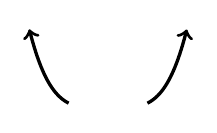
\begin{tikzpicture}
    \draw[very thick, <-] plot [domain=-1:-0.5, samples=50] (\x, {(\x)^4});
    \draw[very thick, ->] plot [domain=0.5:1, samples=50] (\x, {(\x)^4});
\end{tikzpicture} & 
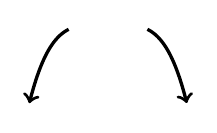
\begin{tikzpicture}
    \draw[very thick, <-] plot [domain=-1:-0.5, samples=50] (\x, {-1*(\x)^4});
    \draw[very thick, ->] plot [domain=0.5:1, samples=50] (\x, {-1*(\x)^4});
\end{tikzpicture} & 
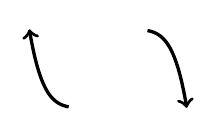
\begin{tikzpicture}
    \draw[very thick, <-] plot [domain=-1:-0.5, samples=50] (\x, {(\x)^6});
    \draw[very thick, ->] plot [domain=0.5:1, samples=50] (\x, {-1*(\x)^6+1});
\end{tikzpicture} & 
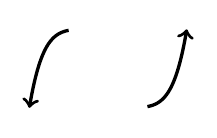
\begin{tikzpicture}
    \draw[very thick, <-] plot [domain=-1:-0.5, samples=50] (\x, {-1*(\x)^6+1});
    \draw[very thick, ->] plot [domain=0.5:1, samples=50] (\x, {(\x)^6});
\end{tikzpicture}\\
\hline
\end{tabular}
\end{center}
\noindent
For each polynomial below, find the following: \\
\textbf{(a)} the degree,
\textbf{(b)} the leading coeffficient, and
\textbf{(c)} the rough sketch of the end behavior\\
\rule[0.5em]{\linewidth}{0.4pt}
\noindent
EX\#1 $f(x) =  -x^2 + 4$ \hspace{2.6cm}
EX\#2 $f(x) =  -x^2 + 4$ \hspace{2.6cm}
EX\#3 $f(x) =  -x^2 + 4$ \\
\\\\\\
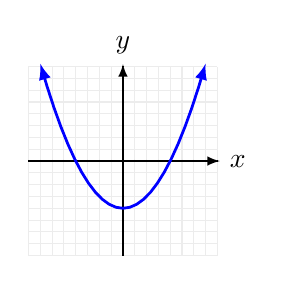
\begin{tikzpicture}[scale=0.15]
        \draw[gray!15,step=1cm] (-8,-8) grid (8,8);
        \draw[line width=0.2mm, -latex] (-8,0) -- (8.2,0) node[right] {$x$};
        % The \foreach loop for x-axis numbers has been modified
        \foreach \x in {-8,...,8} \draw (\x,.1)--(\x,-.1);
        \draw[line width=0.2mm,  -latex] (0,-8) -- (0,8.2) node[above] {$y$};
        % The \foreach loop for y-axis numbers has been modified
        \foreach \y in {-8,...,8} \draw (.1,\y)--(-.1,\y);
        % Blue line with adjusted label 'A'
        \draw[blue,line width=1pt, latex-latex] plot[domain= -7:7] (\x,{0.25*\x*\x-4}) node[font=\tiny] {};    
\end{tikzpicture}
\hspace{3cm}
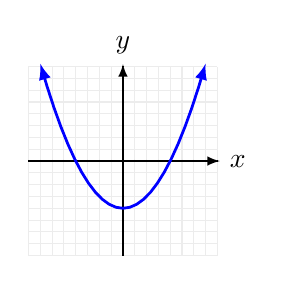
\begin{tikzpicture}[scale=0.15]
        \draw[gray!15,step=1cm] (-8,-8) grid (8,8);
        \draw[line width=0.2mm, -latex] (-8,0) -- (8.2,0) node[right] {$x$};
        % The \foreach loop for x-axis numbers has been modified
        \foreach \x in {-8,...,8} \draw (\x,.1)--(\x,-.1);
        \draw[line width=0.2mm,  -latex] (0,-8) -- (0,8.2) node[above] {$y$};
        % The \foreach loop for y-axis numbers has been modified
        \foreach \y in {-8,...,8} \draw (.1,\y)--(-.1,\y);
        % Blue line with adjusted label 'A'
        \draw[blue,line width=1pt, latex-latex] plot[domain= -7:7] (\x,{0.25*\x*\x-4}) node[font=\tiny] {};    
\end{tikzpicture}
\hspace{3cm}
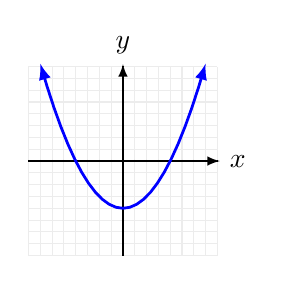
\begin{tikzpicture}[scale=0.15]
        \draw[gray!15,step=1cm] (-8,-8) grid (8,8);
        \draw[line width=0.2mm, -latex] (-8,0) -- (8.2,0) node[right] {$x$};
        % The \foreach loop for x-axis numbers has been modified
        \foreach \x in {-8,...,8} \draw (\x,.1)--(\x,-.1);
        \draw[line width=0.2mm,  -latex] (0,-8) -- (0,8.2) node[above] {$y$};
        % The \foreach loop for y-axis numbers has been modified
        \foreach \y in {-8,...,8} \draw (.1,\y)--(-.1,\y);
        % Blue line with adjusted label 'A'
        \draw[blue,line width=1pt, latex-latex] plot[domain= -7:7] (\x,{0.25*\x*\x-4}) node[font=\tiny] {};    
    \end{tikzpicture}\\\\
\rule[0.5em]{\linewidth}{0.4pt}
\#1 $f(x) =  -x^2 + 4$ \hspace{3cm}
\#2 $f(x) =  -x^2 + 4$ \hspace{3cm}
\#3 $f(x) =  -x^2 + 4$ \\
\\\\\\
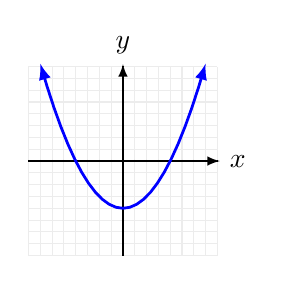
\begin{tikzpicture}[scale=0.15]
        \draw[gray!15,step=1cm] (-8,-8) grid (8,8);
        \draw[line width=0.2mm, -latex] (-8,0) -- (8.2,0) node[right] {$x$};
        % The \foreach loop for x-axis numbers has been modified
        \foreach \x in {-8,...,8} \draw (\x,.1)--(\x,-.1);
        \draw[line width=0.2mm,  -latex] (0,-8) -- (0,8.2) node[above] {$y$};
        % The \foreach loop for y-axis numbers has been modified
        \foreach \y in {-8,...,8} \draw (.1,\y)--(-.1,\y);
        % Blue line with adjusted label 'A'
        \draw[blue,line width=1pt, latex-latex] plot[domain= -7:7] (\x,{0.25*\x*\x-4}) node[font=\tiny] {};    
\end{tikzpicture}
\hspace{3cm}
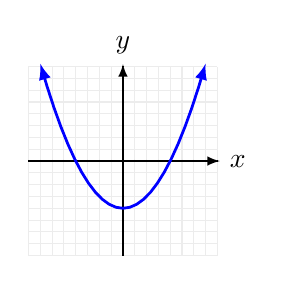
\begin{tikzpicture}[scale=0.15]
        \draw[gray!15,step=1cm] (-8,-8) grid (8,8);
        \draw[line width=0.2mm, -latex] (-8,0) -- (8.2,0) node[right] {$x$};
        % The \foreach loop for x-axis numbers has been modified
        \foreach \x in {-8,...,8} \draw (\x,.1)--(\x,-.1);
        \draw[line width=0.2mm,  -latex] (0,-8) -- (0,8.2) node[above] {$y$};
        % The \foreach loop for y-axis numbers has been modified
        \foreach \y in {-8,...,8} \draw (.1,\y)--(-.1,\y);
        % Blue line with adjusted label 'A'
        \draw[blue,line width=1pt, latex-latex] plot[domain= -7:7] (\x,{0.25*\x*\x-4}) node[font=\tiny] {};    
\end{tikzpicture}
\hspace{3cm}
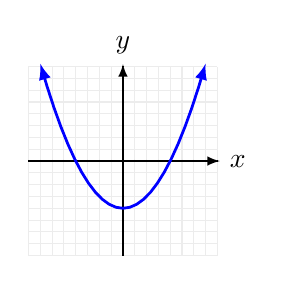
\begin{tikzpicture}[scale=0.15]
        \draw[gray!15,step=1cm] (-8,-8) grid (8,8);
        \draw[line width=0.2mm, -latex] (-8,0) -- (8.2,0) node[right] {$x$};
        % The \foreach loop for x-axis numbers has been modified
        \foreach \x in {-8,...,8} \draw (\x,.1)--(\x,-.1);
        \draw[line width=0.2mm,  -latex] (0,-8) -- (0,8.2) node[above] {$y$};
        % The \foreach loop for y-axis numbers has been modified
        \foreach \y in {-8,...,8} \draw (.1,\y)--(-.1,\y);
        % Blue line with adjusted label 'A'
        \draw[blue,line width=1pt, latex-latex] plot[domain= -7:7] (\x,{0.25*\x*\x-4}) node[font=\tiny] {};    
    \end{tikzpicture}\\\\
\rule[0.5em]{\linewidth}{0.4pt}
\#4 $f(x) =  -x^2 + 4$ \hspace{3cm}
\#5 $f(x) =  -x^2 + 4$ \hspace{3cm}
\#6 $f(x) =  -x^2 + 4$ \\
\\\\\\
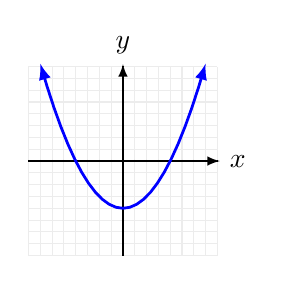
\begin{tikzpicture}[scale=0.15]
        \draw[gray!15,step=1cm] (-8,-8) grid (8,8);
        \draw[line width=0.2mm, -latex] (-8,0) -- (8.2,0) node[right] {$x$};
        % The \foreach loop for x-axis numbers has been modified
        \foreach \x in {-8,...,8} \draw (\x,.1)--(\x,-.1);
        \draw[line width=0.2mm,  -latex] (0,-8) -- (0,8.2) node[above] {$y$};
        % The \foreach loop for y-axis numbers has been modified
        \foreach \y in {-8,...,8} \draw (.1,\y)--(-.1,\y);
        % Blue line with adjusted label 'A'
        \draw[blue,line width=1pt, latex-latex] plot[domain= -7:7] (\x,{0.25*\x*\x-4}) node[font=\tiny] {};    
\end{tikzpicture}
\hspace{3cm}
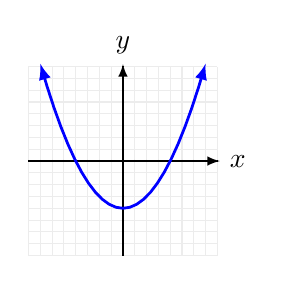
\begin{tikzpicture}[scale=0.15]
        \draw[gray!15,step=1cm] (-8,-8) grid (8,8);
        \draw[line width=0.2mm, -latex] (-8,0) -- (8.2,0) node[right] {$x$};
        % The \foreach loop for x-axis numbers has been modified
        \foreach \x in {-8,...,8} \draw (\x,.1)--(\x,-.1);
        \draw[line width=0.2mm,  -latex] (0,-8) -- (0,8.2) node[above] {$y$};
        % The \foreach loop for y-axis numbers has been modified
        \foreach \y in {-8,...,8} \draw (.1,\y)--(-.1,\y);
        % Blue line with adjusted label 'A'
        \draw[blue,line width=1pt, latex-latex] plot[domain= -7:7] (\x,{0.25*\x*\x-4}) node[font=\tiny] {};    
\end{tikzpicture}
\hspace{3cm}
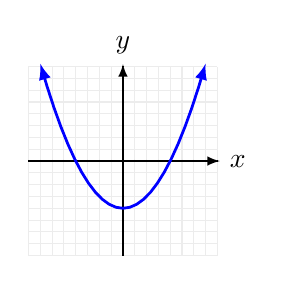
\begin{tikzpicture}[scale=0.15]
        \draw[gray!15,step=1cm] (-8,-8) grid (8,8);
        \draw[line width=0.2mm, -latex] (-8,0) -- (8.2,0) node[right] {$x$};
        % The \foreach loop for x-axis numbers has been modified
        \foreach \x in {-8,...,8} \draw (\x,.1)--(\x,-.1);
        \draw[line width=0.2mm,  -latex] (0,-8) -- (0,8.2) node[above] {$y$};
        % The \foreach loop for y-axis numbers has been modified
        \foreach \y in {-8,...,8} \draw (.1,\y)--(-.1,\y);
        % Blue line with adjusted label 'A'
        \draw[blue,line width=1pt, latex-latex] plot[domain= -7:7] (\x,{0.25*\x*\x-4}) node[font=\tiny] {};    
    \end{tikzpicture}\\
\rule[0.5em]{\linewidth}{0.4pt}
%   also do x to inf and f to inf 
%   match to graph
%   and x to blank f to blank from graph

\end{document}